\chapter[Introdução]{Introdução}

A Cadeira de rodas manual (CRM) é um importante instrumento para a funcionalidade diária na vida daqueles que tem os membros inferiores comprometidos. Segundo uma pesquisa realizada em 2010 pelo IBGE existe cerca de 4,4 milhões de indivíduos incapazes ou com grandes dificuldades de locomoção em todo o Brasil ~\cite{ibge:cartilha:2010}, cadeirantes, em sua maioria.

Segundo Sagawa et al  as CRM são consideradas meios de locomoção de baixa eficiência mecânica (2 a 10\%), além disso os membros superiores não foram preparados para fazerem tantos esforços e movimentos repetidos,  para indivíduos que ainda estão em fase de adaptação esse esforço é ainda maior e para aqueles com sobrepeso os problemas de sobrecarga podem ser tão sérios quanto os riscos cardiovasculares.

Na busca de aumentar a funcionalidade de independência do indivíduo, a cadeira de rodas elétrica surgiu para oferecer a ele maior facilidade e eficácia no deslocamento.

Nesse âmbito, nos últimos anos projetos de automação de cadeiras de rodas manuais ~\cite{brunel:wheelchair:2004}, \cite{artigo_rudi}, \cite{patent_cadeira_rodas_eletrica},	 \cite{marcos:controle:2002}  vem sido testados, estes dão ao cadeirante a facilidade de mobilidade  e ao mesmo tempo utilizam-se do fato de que a cadeira de rodas manual do cadeirante já está com a ergometria  adaptada as necessidades do individuo.

Dessa forma, diante da importância entre a relação homem/cadeira de rodas o presente trabalho tem como objetivo prototipar um kit de automação de cadeira de rodas que seja acoplável a todas as cadeiras de rodas  Para garantir que esse produto seja compatível com o maior número de cadeiras de rodas do mercado possível, seguir-se-á o padrão especificado pela NBR 9050 (ABNT, 2004) e as dimensões do INMETRO~\cite{inmetro}.

\section{Objetivos}
\subsection{Objetivos Gerais}

O principal objetivo desse trabalho é desenvolver um kit de automação de cadeira de rodas, portátil e removível, o que tornará possível descartar o uso do trabalho humano para locomoção da CRM. Para garantir que esse produto seja compatível com o maior número de cadeiras de rodas do mercado, seguir-se-á o padrão especificado pela NBR 9050 (ABNT, 2004) e as dimensões do INMETRO (HTTP://WWW.INMETRO.GOV.BR/, 2015).

Possibilitando assim o oferecimento um custo significantemente reduzido quando comparado a uma cadeira de rodas motorizada e, além disso, a possibilidade de o cadeirante usufruir dos benefícios da cadeira motorizada sem perder a liberdade e ergonomia que o seu modelo manual proporciona.

\subsection{Objetivos Específicos}

O projeto está dividido em quatro ramos: power train, estrutura, controle e interface com o usuário, pretende-se ter envolvimento de todas as engenharias (Automotiva, Eletrônica, Energia e \textit{software}) nos quatro ramos durante toda a execução do projeto.

\textbf{Engenharia Automotiva}

  \begin{enumerate}
    \item Criar um design que permita um acoplamento, visando a ergonomia, peso e dimensionamento do sistema de power train segundo NBR 9050;
    \item Análises de materiais levando em consideração que o produto deve resistir a adiversidades como água, sol, calor, etc.
    \item Análise de esforços;
    \item Montagem do protótipo
  \end{enumerate}

\textbf{Engenharia Eletrônica}
  \begin{enumerate}
    \item Construir um sistema automatizado de controle que seja capaz de gerir as funcionalidades do kit de automação;
    \item Dar condição de pleno funcionamento para o controle de potência e motor utilizando pontes H;
    \item Permitir a interação do usuário com o kit de automação com o uso de periféricos;
    \item Auxiliar no desenvolvimento e criação de interface com o usuário;
  \end{enumerate}

\textbf{Engenharia de Energia}
  \begin{enumerate}
    \item Dimensionamento do motor com o menor requerimento de potência, ou seja, obter uma relação torque-potência ótimo para o sistema de tração elétrica;
    \item Dimensionamento do redutor, visto que motores elétricos CC não possuem o torque necessário para a movimentação da cadeira, visto que motores elétricos CC possuem baixo torque nominal;
    \item Dimensionamento da bateria visando os requisitos: peso, custo, autonomia, e transporte do produto por vias aéreas; e
    \item Desenvolver o melhor sistema de acoplamento entre o motor e a roda do kit afim de que a transmissão de forças seja a mais eficiente possível.
  \end{enumerate}

\textbf{Engenharia de \textit{software}}
  \begin{enumerate}
    \item Montar arquitetura da informação de forma evolutivel e escalonável em relação a qualquer código a ser desenvolvido.
    \item Testar Incrementalmente as unidades usando metodologias TDD e se possível BDD.
    \item Desenvolver incrementalmente de forma a manter a integração continua.
  \end{enumerate}

\section{Estado Técnico}

\subsection{História}
O primeiro meio de suporte para pessoas doentes ou deficientes, possivelmente foi a maca, que foi inventada por volta 4000aC. Ela era leve e podia ser facilmente transportada pelos escravos, servos ou membros da família (SOUZA, 2011).

Uma cama de criança, retratada em um vaso grego do século VI aC, pode ser considerada a mais antiga representação de um veículo sobre roda em ambientes internos. Uma escultura feita mil anos após o vaso, pode ser considerada a mais antiga representação de uma cadeira de rodas. Acredita-se que a escultura venha da China, sendo o único país da metade oriental da Ásia em que as cadeiras foram usadas antes dos tempos modernos (SOUZA, 2011).

No século III dC, foi inventando um veículo muito utilizado até hoje, o carrinho de mão. Este objeto chegou a Europa por volta do século XII dC pela rota das Cruzadas, sendo um veículo útil para todos os tipos de natureza (SOUZA, 2011).

Por volta do século XVI, algumas cadeiras receberam pequenas rodas ou rolos, dando comodidade aos idosos e doentes, onde essas cadeiras tinham as costas reclináveis, apoio de cabeça e apoio de braço. Com a criação dessas cadeiras, os idosos e doentes não precisavam ficar confinados nas camas, já que muitas dessas cadeiras eram feitas individualmente e para a própria utilização do dono (SOUZA, 2011).

Com o passar do tempo, cresceu o desejo pelo conforto, com isso, foram feitos algumas alterações nos contornos das cadeiras, onde elas recebiam braços adaptados às formas do corpo humano. Entretanto, as cadeiras de rodas ainda precisavam de alguma pessoa para empurrar. Uma das últimas melhorias que foi aplicada às cadeiras de rodas, foi no final do século XIX, quando as rodas de bicicletas de madeira foram substituídas por raios de metais, deixando-as bem parecidas com as que usamos hoje em dia. Um pouco mais tarde, quando as rodas de bicicletas foram envoltas com pneu de borracha, os fabricantes das cadeiras de rodas começaram a seguir essa tendência (SOUZA, 2011).

No início do século XX, o inventor americano George Westinghouse, fez alguns desenhos sobre suas idéias para a criação de uma cadeira de rodas elétrica, entretanto, Westinghouse faleceu em 1914 sem ter construído uma cadeira de rodas elétrica. Apesar disso, muitos o consideram como o inventor da cadeira de rodas elétrica. Alguns anos depois, um grupo de engenheiros criou uma cadeira de rodas motorizada, entretanto, esta era muito cara, pesada e inflexível para os consumidores (CLARK, 1997), (SHEPARD; KAREN,1984).

Já no início da década de 1930, Harry Jennings projetou uma cadeira de rodas dobrável com a ajuda de um paraplégico, o que acabou melhorando os modelos seguintes das cadeiras de rodas elétricas (CLARK, 1997), (SHEPARD; KAREN, 1984).
De acordo com a necessidade e avanço cientifico e tecnológico do ser humano as cadeiras de rodas se tornaram um novo produto. Visando o mercado, várias empresas investiram na fabricação e desenvolvimento de modelos e tecnologias, que beneficiam aos cadeirantes. Existem atualmente diversos modelos de cadeiras de roda como cadeiras para banhos, cadeiras automatizadas, cadeiras dobráveis é até mesmo kits de automação, equipamentos que se tornaram de extrema importância para facilitar a acessibilidade dos cadeirantes (HTTP://WWW.SCIELO.BR/PDF/PROD/V12N1/V12N1A06, 2012).

\subsection{O Estado da Arte}

As tecnologias Assistivas, que são recursos tecnológicos que facilitam a vida das pessoas com algum tipo de deficiência, tem se tornado hoje um assunto cada vez mais comum. O avanço tecnológico tem facilitado para que haja uma inclusão social cada vez maior auxiliando atividades como: a automação de ambientes, que facilita para a execução de tarefas simples; na correção postural, com cadeiras que beneficiam a postura de pessoas que possuem alguma deficiência física; e na locomoção, que podem ser bengalas, cadeiras de rodas manuais ou elétricas, qualquer equipamento ou estratégia que auxilie na mobilidade.

A NBR9050 recomenda padrões de cadeiras de roda manuais e ajustes estruturais da mobília para de prédios para acessibilidade de pessoas com deficiência, estabelecendo padrões de estofados, dimensões estruturais, dentre outros que facilitam a vida de pessoas com deficiência (BECKER, 2000).

Hoje em dia, com a tecnologia mais avançada e os estudos em materiais mais resistentes e leves, pode-se observar uma vasta gama de cadeiras de rodas manuais e elétricas.

\begin{figure}[!htb]
  \centering
  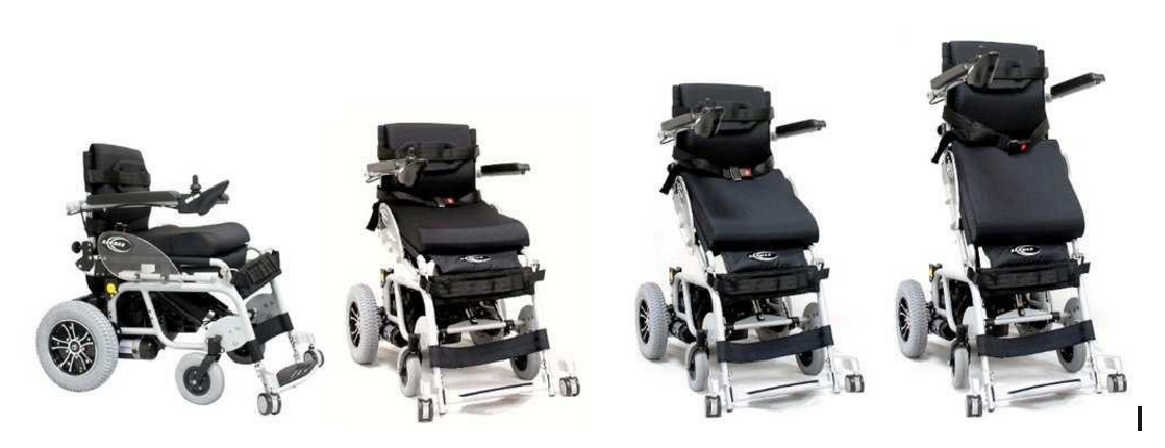
\includegraphics[keepaspectratio=true,scale=0.50]{figuras/introducao/versoes}
  \caption{Cadeira Stand-up}
  \label{fig:stand_up}
\end{figure}


Na figura \ref{fig:stand_up}, é apresentado uma cadeira de rodas do modelo stand-up, em que existem modelos manuais e motorizadas. Seu principal objetivo para o cadeirante é melhorar sua auto-estima, facilitando a acessibilidade nas atividades cotidianas, como exemplo, pegar um livro em uma estante, ou simplesmente olhar uma pessoa frente a frente. Isso ocorre devido a cadeira ter um sistema de elevação elétrico ou manual, permitindo pequenos deslocamentos do corpo da pessoa na posição ereta, com segurança e praticidade (HTTP://WWW.CAVENAGHI.COM.BR/, 2015).

\begin{figure}[!htb]
  \centering
  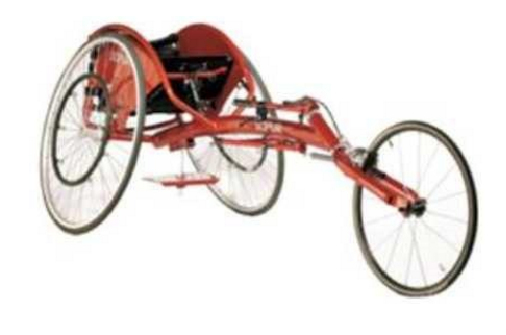
\includegraphics[keepaspectratio=true,scale=0.50]{figuras/introducao/cadeira_desporte}
  \caption{Cadeira desporto}
  \label{fig:desporto}
\end{figure}


Na figura \ref{fig:desporto}, tem um exemplo de cadeira de rodas para desporto. Esse tipo de cadeira de rodas são utilizadas nas atividades desportivas, onde cada cadeira é feita de acordo com a deficiência do para-atleta. Essas cadeiras são feitas com materiais leves, para que o para atleta tenha mais velocidade e mobilidade (FREIRE, 2009).

Na figura \ref{fig:kit_motorizacao} é apresentado a patente (PI0304753-9), que é um kit para motorização de cadeiras de rodas, em que as rodas de uma cadeira de rodas manual será tracionada por um conjunto de rodas menores comandadas por um joystick. Na figura também é possível visualizar a presença de um joystick fixado junto ao apoio de braço direito. Cabe ressaltar que este Joystick pode ser acoplado do lado esquerdo da cadeira de rodas (HTTP://WWW.PATENTESONLINE.COM.BR/,2015).

\begin{figure}[!htb]
  \centering
  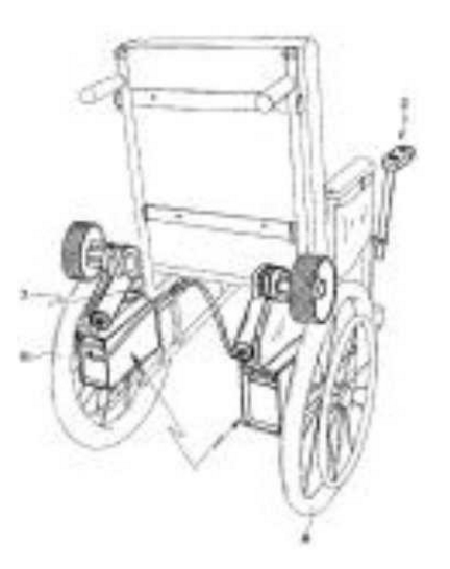
\includegraphics[keepaspectratio=true,scale=0.50]{figuras/introducao/kit_motorizacao}
  \caption{Patente de um kit de automação de cadeiras de rodas}
  \label{fig:kit_motorizacao}
\end{figure}

A idéia dessa patente serviu de inspiração para o desenvolvimento desse projeto, onde a idéia principal é construir um kit para ser acoplado em qualquer cadeira de rodas manual, transformando-a em motorizada.

\section{Requisitos}

Os requisitos iniciais do projeto foram definidos a fim de facilitar um planejamento na fase inicial, ajudar na definição das tecnologias que serão utilizadas, e gerenciamento do projeto.

\subsection{Requisitos em Relação a Estrutura}

  \begin{itemize}
    \item O sistema de acoplamento entre o kit de automação e a cadeira deve ser universal com base nas do dimensões do INMETRO;
    \item O projeto de design deve ser discreto;
    \item A ergonomia do kit deve prover conforto e segurança ao usuário;
    \item Transmissão de torque e potência entre o kit e a roda da cadeira de rodas deve possuir as menores perdas possíveis;
    \item O peso do conjunto motor-bateria deve ser o menor possível. Esse requisito está também atrelado ao custo- benefício.

  \end{itemize}

\subsection{Requisitos em Relação as Tecnologias}

  \begin{itemize}
    \item É necessário um sistema de automação, controle dos motores, indicadores e controladores de potência;
    \item Interface com o usuário deve ser simples e acessível;
    \item A velocidade mínima da comunicação entre interface do usuário e placas de controle deve ser a mais alta possível. \item Este requisito será melhor adequado em relação a valores assim que testado com o usuário.
  \end{itemize}

\subsection{Requisitos em Relação a Parte Financeira}
  \begin{itemize}
    \item Os custos totais do protótipo devem ser consideravelmente menores aos de uma cadeira de rodas motorizada;
    \item Os custo-benefício das peças a serem utilizadas no projeto devem ser embasados em cálculos matemáticos de quantidade-analisada por valor a ser pago.
  \end{itemize}
